
\section{Oscilloscopio}

Unendo tutte le funzionalità spiegate in precedenza, siamo in grado di usare il microcontrollore come oscilloscopio. Per farlo, però, serve un meccanismo di trigger che ci permetta di selezionare solo i segnali voluti.

\subsection{Trigger}
Sono stati sperimentati diversi tipi di trigger con diverse periferiche. In particolare, i trigger utilizzati sono:
\begin{itemize}
    \item Trigger a singola soglia software: Un trigger che usando il software controlla se il valore misurato è maggiore di una soglia
    \item Trigger a singola soglia hardware: Un trigger che usando un comparatore hardware controlla se il valore misurato è maggiore di una soglia
    \item Trigger in salita software: Un trigger che controlla prima se il valore è sotto una soglia e poi se un valore successivo è sopra un'altra soglia. Questo trigger permette di evitare di triggerare in discesa e quindi quando il segnale è già passato.
    \item Trigger in salita hardware: Un trigger basato sul controllo precedente ma fatto con dei comparatori al posto che dal software.
\end{itemize}

\subsubsection{Trigger a singola soglia software}
Questo tipo di trigger corrisponde alla versione più semplice ed intuitiva di trigger. Il microcontrollore per controllare il valore deve fare diverse operazioni e questo rallenta notevolmente il codice. Inoltre, questo tipo di trigger non permette di selezionare con precisione il segnale desiderato, in quanto per ogni soglia scelta diversa dal picco massimo del segnale, il segnale potrebbe triggerare in 2 momenti diversi.

\noindent
\begin{minted}[bgcolor=coding , linenos]{C}
uint8_t flag_Trigger_EN = 0;
uint8_t flag_Triggered = 0;

void ESPE_DMA_Trigger(void){
    if(!flag_Triggered && flag_Trigger_EN){ // Se non è già stato triggerato
                                            //e è arrivato il segnale di attivazione
                                            //del trigger
        if( ADC3 -> DR > Trigger_Value){ // Se il valore è maggiore della soglia
            flag_Triggered = 1; // Triggerato
            flag_Trigger_EN = 0; //Reset Flag
        }
    }
}
\end{minted}

\subsubsection{Trigger in salita software}
Il trigger in salita è una diretta evoluzione del trigger a singola soglia. Infatti, la presenza di 2 soglie di riferimento che agiscono in momenti diversi del segnale, permette di avere un trigger più preciso e affidabile. Questo trigger, però, è molto più complesso da implementare e richiede un controllo molto più preciso del segnale. Inoltre, seppur di poco rallenta il codice in quanto il numero di operazioni aumenta.

\begin{wrapfigure}{l}{0.5\linewidth}
    \centering
    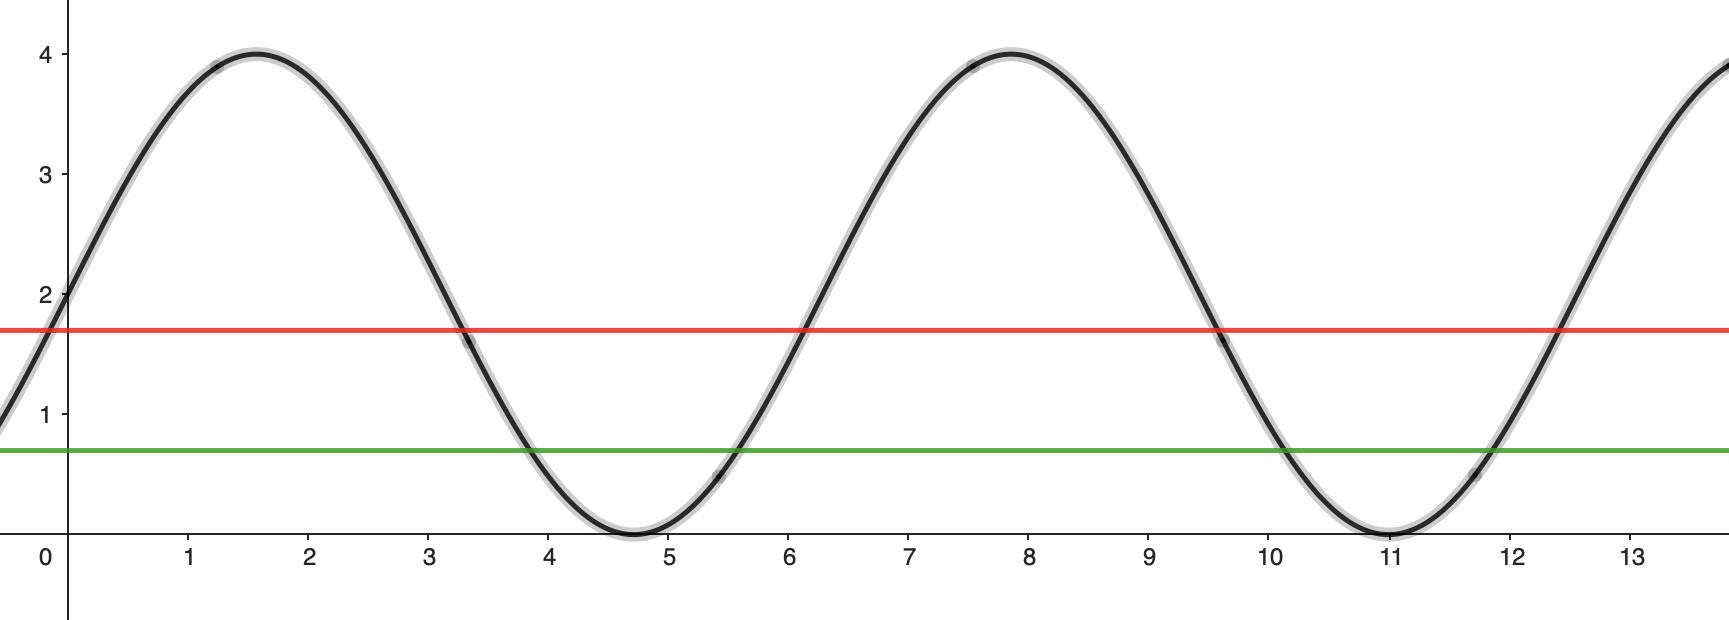
\includegraphics[width=\linewidth]{oscilloscopio/assets/trigger.png}
    \caption{Trigger in salita}
    \label{fig:Trigger}
\end{wrapfigure}

Come si vede dalla figura \hypersetup{linkcolor=black}{\ref{fig:Trigger}}, se si controlla prima se il segnale è sotto la linea verde, o \textit{Soglia di Pretrigger} e poi si controlla se il segnale è sopra la linea rossa, o \textit{Soglia di Trigger}, si può risolvere il problema di ambiguità che c'era nel trigger a singola soglia. Questo processo rende molto più costante il trigger e permette di selezionare con precisione il segnale desiderato.
Invertendo il processo, si ottiene il trigger in discesa, il quale permette di selezionare il punto che è stato scartato in questo caso.\\

A livello di programmazione, questo codice è leggermente più complesso del precedente, ma ci permette di gestire i dati con una precisione migliore. Infatti con questo codice possiamo sceglere anche di prenderer i dati prima del trigger, scegliendo con precisione il punto in cui iniziare a prendere i dati.

\noindent
\begin{minted}[bgcolor=coding , linenos]{C}
uint8_t flag_Trigger_EN = 0;
uint8_t flag_Triggered = 0;
uint8_t flag_Pretriggered = 0;
int index = 0;
int index_stop = 0;


void ESPE_DMA_Trigger_Pretrigger(void){
    if(!flag_Triggered && flag_Trigger_EN){ // Se non è già stato
                                                        //triggerato e è arrivato
                                                        //il segnale di attivazione
                                                        //del trigger
        if( flag_Pretriggered){ // Se il segnale è stato pretriggerato
            if( ADC3 -> DR > Trigger_Value){ // Se il valore è maggiore della
                                            //soglia di trigger
                flag_Triggered = 1; // Triggerato
                flag_Trigger_EN = 0; //Resetta i Flag
                flag_Pretriggered = 0;
                index = vec_len - DMA1_Stream0 -> NDTR + data_len +1
                index_stop = vec_len - (index)%vec_len; //Calcola l'indice di stop
            }
            return;
        }
        if( ADC3 -> DR < Pretrigger_Value){ // Se il valore è minore della soglia
                                            //di pretrigger
            flag_Pretriggered = 1; // Pretriggerato
        }
    }
}
\end{minted}

\subsubsection{Trigger hardware}
Entrambi i trigger Hardware, non sono altro che variazioni dei trigger software a cui, al posto di controllare la soglia con un if, si usa un valore all'interno del registro del microcontrollore. Questo passaggio permette di saltare la conversione del valore fatta dall'ADC e di avere solo un valore booleano.


Per quanto riguarda il trigger hadware a singola soglia:
\noindent
\begin{minted}[bgcolor=coding , linenos]{C}
uint8_t flag_Trigger_EN = 0;
uint8_t flag_Triggered = 0;

void ESPE_DMA_COMP_Trigger(void){
if(!flag_Triggered && flag_Trigger_EN ){// Se non è già stato triggerato e è arrivato
                                            //il segnale di attivazione del trigger
        if( COMP12 -> SR & COMP_SR_C2VAL ){ // Se il comparatore ha triggerato
            flag_Triggered = 1; // Triggerato
            flag_Trigger_EN = 0; //Reset Flag
        }
    }
}
\end{minted}

Il trigger in salita Hardware, è possibile farlo con un singolo comparatore al posto di 2 usando l'Isteresi. Questo comportamento anomalo dei comparatori reali, permette una sottile divisione dal voltaggio di quando il comparatore è triggerato e quando non lo è. Usando questo comportamento come pretrigger, si evita di aggiungere cavi per un altro comparatore. Cosa che si deve comunque fare nel caso in cui si voglia un pretrigger notevolmente più basso del trigger.

\noindent
\begin{minted}[bgcolor=coding , linenos]{C}
void ESPE_DMA_COMP_Trigger_Pretrigger(void){
if(!flag_Triggered && flag_Trigger_EN){
    if( flag_Pretriggered){
        if( COMP12 -> SR & COMP_SR_C2VAL){
            flag_Triggered = 1;
            flag_Trigger_EN = 0;
            flag_Pretriggered = 0;
            index_stop = vec_len - (vec_len - DMA1_Stream0 -> NDTR + data_len +1)%vec_len;
        }
        return;
    }
    if( !(COMP12-> SR & COMP_SR_C2VAL) ){
        flag_Pretriggered = 1;
    }
}
}
\end{minted}

Il lato negativo del trigger hardware è la quantità di cavi da collegare al microcontrollore. Infatti, per ogni comparatore che si vuole usare, c'è bisogno di 2 cavi aggiuntivi in parallelo con quelli collegati all'ADC. Se si sta lavorando ad alta frequenza o con tanti cavi, questo può causare una deformazione dell'onda.

Velocizzando tutti i processi al massimo, si ottiene un oscilloscopio in grado di misurare segnali fino a 30MHz.\\